\documentclass{sigchi}

% Use this command to override the default ACM copyright statement
% (e.g. for preprints).  Consult the conference website for the
% camera-ready copyright statement.

%% EXAMPLE BEGIN -- HOW TO OVERRIDE THE DEFAULT COPYRIGHT STRIP -- (July 22, 2013 - Paul Baumann)
% \toappear{Permission to make digital or hard copies of all or part of this work for personal or classroom use is      granted without fee provided that copies are not made or distributed for profit or commercial advantage and that copies bear this notice and the full citation on the first page. Copyrights for components of this work owned by others than ACM must be honored. Abstracting with credit is permitted. To copy otherwise, or republish, to post on servers or to redistribute to lists, requires prior specific permission and/or a fee. Request permissions from permissions@acm.org. \\
% {\emph{CHI'14}}, April 26--May 1, 2014, Toronto, Canada. \\
% Copyright \copyright~2014 ACM ISBN/14/04...\$15.00. \\
% DOI string from ACM form confirmation}
%% EXAMPLE END -- HOW TO OVERRIDE THE DEFAULT COPYRIGHT STRIP -- (July 22, 2013 - Paul Baumann)

% Arabic page numbers for submission.  Remove this line to eliminate
% page numbers for the camera ready copy
% \pagenumbering{arabic}

% Load basic packages
\usepackage{balance}  % to better equalize the last page
\usepackage{graphics} % for EPS, load graphicx instead 
\usepackage[T1]{fontenc}
\usepackage{txfonts}
\usepackage{mathptmx}
\usepackage[pdftex]{hyperref}
\usepackage{color}
\usepackage{booktabs}
\usepackage{textcomp}
% Some optional stuff you might like/need.
\usepackage{microtype} % Improved Tracking and Kerning
% \usepackage[all]{hypcap}  % Fixes bug in hyperref caption linking
\usepackage{ccicons}  % Cite your images correctly!
% \usepackage[utf8]{inputenc} % for a UTF8 editor only

% If you want to use todo notes, marginpars etc. during creation of your draft document, you
% have to enable the "chi_draft" option for the document class. To do this, change the very first
% line to: "\documentclass[chi_draft]{sigchi}". You can then place todo notes by using the "\todo{...}"
% command. Make sure to disable the draft option again before submitting your final document.
\usepackage{todonotes}

% Paper metadata (use plain text, for PDF inclusion and later
% re-using, if desired).  Use \emtpyauthor when submitting for review
% so you remain anonymous.
\def\plaintitle{Crowd-Aware Co-design of Floor Plans using Simulation Guided Games }
\def\plainauthor{First Author, Second Author, Third Author,
	Fourth Author, Fifth Author}
\def\emptyauthor{}
\def\plainkeywords{Architectural Design;Crowd-aware;Gamification;Co-Design.}
\def\plaingeneralterms{Graphics, Games, Design, Crowd Simulation}

% llt: Define a global style for URLs, rather that the default one
\makeatletter
\def\url@leostyle{%
	\@ifundefined{selectfont}{
		\def\UrlFont{\sf}
	}{
	\def\UrlFont{\small\bf\ttfamily}
}}
\makeatother
\urlstyle{leo}

% To make various LaTeX processors do the right thing with page size.
\def\pprw{8.5in}
\def\pprh{11in}
\special{papersize=\pprw,\pprh}
\setlength{\paperwidth}{\pprw}
\setlength{\paperheight}{\pprh}
\setlength{\pdfpagewidth}{\pprw}
\setlength{\pdfpageheight}{\pprh}

% Make sure hyperref comes last of your loaded packages, to give it a
% fighting chance of not being over-written, since its job is to
% redefine many LaTeX commands.
\definecolor{linkColor}{RGB}{6,125,233}
\hypersetup{%
	pdftitle={\plaintitle},
	% Use \plainauthor for final version.
	%  pdfauthor={\plainauthor},
	pdfauthor={\emptyauthor},
	pdfkeywords={\plainkeywords},
	bookmarksnumbered,
	pdfstartview={FitH},
	colorlinks,
	citecolor=black,
	filecolor=black,
	linkcolor=black,
	urlcolor=linkColor,
	breaklinks=true,
}

% create a shortcut to typeset table headings
% \newcommand\tabhead[1]{\small\textbf{#1}}

% End of preamble. Here it comes the document.
\begin{document}
\newcommand{\red}[1]{\textcolor{red}{#1}}
\newcommand{\draft}[1]{\textcolor{blue}{#1}}


\title{\plaintitle}

%\numberofauthors{5}
%\author{%
%	\alignauthor{Leave Authors Anonymous\\
%		\affaddr{for Submission}\\
%		\affaddr{City, Country}\\
%		\email{e-mail address}}\\
%	\alignauthor{Leave Authors Anonymous\\
%		\affaddr{for Submission}\\
%		\affaddr{City, Country}\\
%		\email{e-mail address}}\\
%	\alignauthor{Leave Authors Anonymous\\
%		\affaddr{for Submission}\\
%		\affaddr{City, Country}\\
%		\email{e-mail address}}\\
%}

\maketitle

\begin{figure*}
 	\includegraphics[width=\textwidth]{images/FinalTeaser}
 	\caption{(a) Placement of architectural elements, (b) Orthographic view of layout, (c) Visual representation of crowd configuration, (d) Orthographic view of crowd simulation, (e) User evacuation towards exit (g) Modification of layout, (h) Game level example}
\end{figure*}

\begin{abstract}
Architectural design decisions stand to benefit by accounting for the presence and activities of human crowds that inhabit these spaces.  Computational methods for simulating synthetic crowds provide a cost effective means of exploring and analysing the design search space.  However, crowd-aware architectural design is a complex combinatorial decision process, where small changes in the design solution may affect crowds and their flow patterns in unexpected and potentially unintuitive ways. Existing solutions rely on expert intuition or automation, but are unable to account for many contradicting, and often subjective properties while optimizing designs. A single solution approach may also miss potential design solutions that achieve the desired objective specifications, while meeting subjective criteria.  We propose a means of combining these methods in a gamified framework. Using our system, ``players"  (novice users or experts) can rapidly iterate on their designs while soliciting feedback from computer simulations of crowd movement, as well as the designs of previous players. Our approach affords a new way of thinking of the solution space in that it inherently supports competitive co-design and crowd sourced solutions.  We evaluate our framework through a user study and demonstrate the potential of crowd-aware co-design of environments using simulation guided multiplayer games.
\end{abstract}

\category{J.5}{Arts and Humanities}{Architecture} \category{J.6}{Computer-Aided Engineering}{Computer-aided Design} 
\category{K.8.1}{Personal Computing}{Games} 

\keywords{\plainkeywords}

%\conceptlist

%\printcopyright

%%%%%%%%%%%%%%%%%%%%%%%%%%%%%%%
\section{Introduction}
\label{section-introduction}
Designing an architectural or urban plan is a complex problem in which a good solution is one that balances aesthetics, functionality, utilization, and safety of a structure. This makes the problem inherently multiobjective and the solution space combinatorial.  Incorporating the dynamics of large groups of people, or crowds, further complicate the solution space and is prohibitively expensive to do with real people.  Thus layout designs are commonly tested using synthetic crowds that model realistic behaviours under different conditions.  In particular, a layout's performance is most critical during dangerous situations such as evacuations, so these scenarios are used to stress test environments.

Popular architectural design tools such as Autodesk Revit and Rhino3D do not account for evacuation planning or crowd-aware stress testing. There are tools used to analyze a design with simulated crowds, but none of those tool have an integrated environment for both architectural design and crowd simulation. Together these tools are quite complex an require years of training and architectural and safety knowledge.

Fully automated computational solutions for crowd-aware architectural design may miss solutions which are technically sound, crowd-aware, and aesthetically pleasing.  These are highly dependant on the quality of the objective functions for each of these requirements. Recent work in this field has sought for user-in-the-loop optimization processes which make up for these shortcoming and provide the user more control over solution directions.

Our solution is to gamify the process of optimal layout design for crowd-aware architectures, or environments. This game provides the player with feedback in terms of crowd simulation and heatmaps of evacuation dynamics, while affording them editing power within the constraints imposed by the architect or designer. The approach of gamifying complicated problems affords many benefits to both the process and the solution. The most immediate is that the game provides a fun and interactive platform for architectural and urban planning. 

By providing a means to implement the design process as gamified levels with built in architectural constraints, a planner, environment designer, or architect can convert their design problem into a playable game.  This reimagines the architect or planner seeking a design solution as a game maker.

Furthermore, providing the game via the internet, or large scale network of collaborators, design solutions may be crowd sourced.  A user with any level of knowledge in a related field can produce an optimal design plan. This can also be used as a exciting learning platform in the field of architectural education. 

Providing the results of other players designs and their fitness affords a further level of colaboration in the form of competitive co-design.  The collective knowledge of the crowd, as in collaborators, and iterative improvement of co-design will help the layout to converge towards optimality. 

%%%%%%%%%%%%%%%%%%%%%%%%%%%%%%%
\section{Related Work}
\label{section-related-work}
There is an established and growing interest in the use of architectural optimization to explore design spaces and provide optimal solutions with respect to problem criteria~\cite{block2014advances,pottmann2014architectural}. While there are popular CAD solution tools, such as Autodesk Revit and Rhino3D, these tools do not account for crowd behaviour and require significant training and background knowledge. Architectural optimization solutions generate new layouts or topology for structures with respect to objective and/or subjective criteria, while providing a trade off between automation and author precision.  Data driven approaches~\cite{Merrell:2010:CRB:1882261.1866203} learn layout configurations from a database of prior architecture design constrained to a particular design space (e.g., residential homes). In another approach Design objectives can be modelled as forces applied to a physical features to generate layout designs automatically~\cite{arvin2002modeling}.

\red{Some editing has been done here to remove generic references (like theses).  THis section should be about either crowd aware optimization OR crowd simulation, and NOT both}~There are lot of existing research on crowd simulation. The Social Force model allows for highly representative models of human behaviour in simple situations that elicit reflexive reactions~\cite{PhysRevE.51.4282}. The most closely related to our work is the optimization of egress environments using crowds~\cite{johansson2007pedestrian,jiang2014obstacle}. This work does not incorporate the user-in-the-loop processes and is presented as analysis of the affects of egress obstacles and shapes on crowd evacuation. Since subjective criteria are difficult or impossible to quantify, many tools select an optimization scheme to meet objective criteria and then take a human-in-the-loop interactive approach to the subjective. The tools combine the aforementioned derivations for fitness with user guided optimization processes ~\cite{shi2013performance,turrin2011design,Michalek02interactivedesign}. 

\red{THis and the previous paragraph are not grouped properly, we have crowd simulation from generic overview (badler book) to specific (sf + ppr +etc), crowd aware optimization, and then parameter fitting blended over two paragraphs - there should be three separately with clear focus}~The maturity of research in simulating crowd dynamics~\cite{badlerBook,DBLP:books/daglib/0030710} has resulted in a wide variety of approaches including social forces~\cite{helbing2000simulating} and predictive models~\cite{ORCA,ppr}. There has been a growing recent trend to use statistical analysis in the evaluation and analysis of dense crowd simulations.  The work in~\cite{guy2012statistical,Pettre:2009:EMS:1599470.1599495} measures the ability of a steering algorithm to emulate the behavior of a real crowd data set by measuring its divergence from ground truth.  Crowd optimization techniques~\cite{paramFitting,sca.20141129} automatically fit the parameters of a crowd to meet different criteria, or even match real crowds. 

\red{Cite LoS paper here somewhere in terms of the combinatorial decision space of the non-convex optimization problem that is architectural optimization.  Also, cite previous CAVW paper on environment optimization.}

We leverage these wealth of research in crowd simulation to present a computational design tool for environments that uses features extracted from an underlying crowd simulator as criteria for architectural optimization.

There is a plethora of research on crowd simulation and crowd evacuation using serious games. Most closest to our approach is  ~\cite{ribeiro2013towards} where serious games are used to training, planning and evaluating emergency plans but the research more focuses on crowd simulation component than architectural planning. Our Game focuses on optimizing the architectural design keeping in consideration the emergency situation using best suited simulated crowd. So that we can prevent a disaster at an earlier stage. Our game also considers the  research paper~\cite{berseth2014characterizing} for characterizing and optimizing game level difficulty for our architectural planning game~\red{"considers" how?}.

%%%%%%%%%%%%%%%%%%%%%%%%%%%%%%%
\section{Framework Overview}
\label{section-framework}
\begin{figure*}
	\centering  \includegraphics[width=\textwidth]{images/Framework/FrameworkOverview.png}
	\caption{\label{fig:framework-overview}The Game Framework overview}
\end{figure*}

The game design gives players the tools to construct, modify, and analyze environment designs.  A player can add elements to the provided floor design, such as doors, walls, and pillars. The player's goal, and success criteria, is to create an efficient design that evacuates all agents in the shortest possible time. The player can visualize the simulation and analyze the aggregate crowd dynamics using heat maps to identify regions for improvement. The player can use these metrics to improve the current design. By repeating a level and improving the evacuation time, the level layout can converge to an optimal design.

The following list provides an overview of the modules in the framework. The modules and their relationships are also outlined in Figure~\ref{fig:framework-overview}.

\begin{itemize} 
\item \textbf{Static Initial Layout} - A architect or designer can designate static elements of the gamified environment - partially imposing architectural constraints. The player can not modify these elements in the existing layout. Users will have to place the elements provided to this layout. It is possible for the architect or designer to design each subsequent level such that the environment has increased complexity of the existing design or is adds portions to the design.  This means a player may work on a larger environment in which they can modify a portion, or the player may work from the micro to macroscopic portions of a larger design task.

\item \textbf{Player Modified Layout} - There are certain elements available to the user to add to the layout. There are several elements which may be added or modified such as walls, pillars, and doors. Access to these modification and creation tools may be constrained by the architect or designer. 

\item \textbf{Crowd Behaviour Configuration} - The player can configure the different 
characteristics of the crowd to capture new behaviours and dynamics for which the environments fitness is tested in terms of evacuation.  A summary of these crowd parameters are listed below, in depth details are provided in the Crowd Configuration and Simulation Section - 

\begin{enumerate}
\item \textbf{Level of Service (LoS)} - The number of people in a square unit of area that spawn when the level starts, or crowd density.

\item \textbf{Level of Aggression} - The distribution of crowd member speed and acceleration.

\item \textbf{Level of Homogeneity} - The distribution of crowd member width, or size.
\end{enumerate}

These parameters provide players with up to 54 unique combinations of crowd behaviour and dynamics.

\item \textbf{Crowd Simulation} - Once the player finalizes their environment configurations, they can run the simulation. The crowd will begin evacuating the layout towards exits defined by the architect or designer. An agent based model using Unity3D is used for agent steering. The Unity 3D Mechanim system handles character animation and the Navmesh system handles path finding. Once the entire crowd reaches their destination, the simulation ends.

\item \textbf{Validation} - Once the simulation ends, the game displays the score based on the total evacuation time. The winning criteria, lower total evacuation time, determines where in the leader board the player is placed. In this phase, the player can visualize and analyze their results, in terms of crowd dynamics, using heat maps.

\item \textbf{Co-Design} - Players are given the ability to view other players designs and their performances. They may use various analytics to improve designs from a high scoring player. Co-design allows the design task to be tackled from multiple perspectives while converging on optimal designs.
\end{itemize}

%%%%%%%%%%%%%%%%%%%%%%%%%%%%%%%
\section{Encoding architectural standards}
\label{section-environment}
\begin{figure*} \includegraphics[width=\textwidth,height=100pt]{images/1111}
	\caption{Environment Design: a) Invalid wall placement, b)valid wall \& pillar placement, c)Door placement,d) Example of constraints}  
\end{figure*}

The intention of gamifying architectural design is make the game usable by a player with any level of architectural knowledge. To meet these ends, the game framework provides a means of specifying and designing constraints/rules in the layout design phase of our game such that even casual player can achieve a layout which follows architectural standards.

Any architectural layout primarily comprises of walls, pillars, and doors. Hence we provide the tools to the the player to modify and create these elements in the layout. However, the game also provides the tools to create gamified levels with different forms of challenges. An architect or designer may choose to focus on an entire design, and formulate levels in terms constraints on available elements and modifications in increasing levels of difficulty.  The architect or designer may formulate levels in terms of seperate portions of a larger environment and sort them in increasing difficulty, e.g. from the bathroom area, to a common area, to a high traffic area, and so on. The architect or designer may also choose to iteratively incorporate more portions of the environment such that success criteria in the new level may be additive in terms of the previous design.  The gamification framework and level specification affords a number of options in order to lead player to producing designs for the architect or designer.  Display messages can be provided to help casual players learn about architectural standards when their design violate these constraints. Thus, the game can be used not just to produce design but also as an educational tool for novice designers or casual players.


%%%%%%%%%%%%%%%%%%%%%%%%%%%%%%%
\section{Crowd Configuration and Simulation}
\label{section-crowd}
To afford accurate crowd animations for player visualization, a humanoid character model with animations is employed. The complete set includes idle and walking animations. The crowd members are generated and distributed at random locations in the layout based on the configurations set by the player. Destinations and distributions for locations of crowd members can be modified and constrained by the architect or designer as well. To ensure accurate navigation, the navigation mesh of the environment and path plans for each member are recomputed after every level change and before a simulation is started.

We used an agent-based model for simulating crowd steering. We have also tried to incorporate different steering decision behaviours observed in the crowd at the time of emergencies. For instance during a fire, people tend to follow each other in order to find the exits or people tend to follow the exit signs more stringently than in their day to day lives. While going to their destination, if an member sees an exit which is closer than their assigned one their navigation goal switches to the closer observed goal. The members also change their destination and path when a big group of other members are moving towards a certain destination. So in a sense, the members follow the crowd unless they themselves see an exit.

To afford rigorous and complete testing across dynamics and behaviours, the crowds are parametrized for aggression, homogeneity, and density.  These parametrizations and a formal definition of a crowd are provided in the rest of this section.

\begin{itemize}

\item \textbf{Level of Aggression (LoA)} - Three degrees of aggression are provided; low, medium and high. The aggression degree determines the speed and acceleration of different members in the crowd. As the aggression level increases, the distribution of aggressive people in the crowd also increases. Fixed probabilities are associated with the low, medium, and high degrees and are used to assign appropriate speeds to the members. The mapping of degrees of aggression to speeds and accelerations can be seen in Table~\ref{table:aggression-levels-speeds} and Table~\ref{table:aggression-levels-accels} respectively.

\item \textbf{Level of Homogeneity (LoH)} - Three classes of homogeneity are available to the player: low, medium, and high. Changing this configuration changes the distribution of the radii of the crowd members.  Low means that there is a low probability in the variety of members that have a radius other than the average one. This helps the player to identify how well their design handles different body shapes in a crowd.

\item \textbf{Level of Service (LoS)} - There are six Levels of Service available to the player. Level of Service is used by traffic engineers to measure the quality of traffic flow both for automotive and pedestrian applications. LoS classes are typically given a grade level (from A-F), which are summarized in Table~\ref{table:los}. 

\end{itemize}

Examples of these parametrizations can be seen in Figure~\ref{fig:crowd-parameter-ex}.

\begin{figure*} 
	\begin{tabular}{c c c} 
	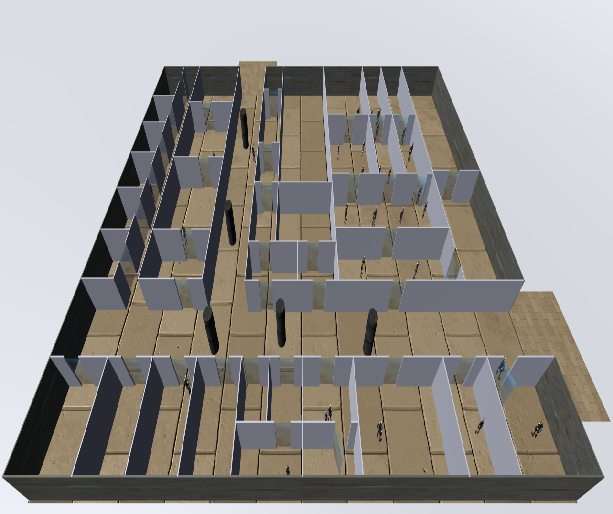
\includegraphics[width=0.31\textwidth]{images/LoS_A_lowest_density.png} & 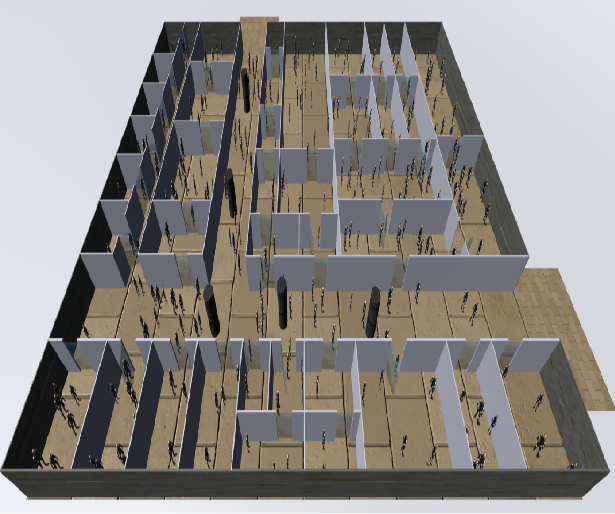
\includegraphics[width=0.31\textwidth]{images/LoS_F_highest_crowd_density.png} & 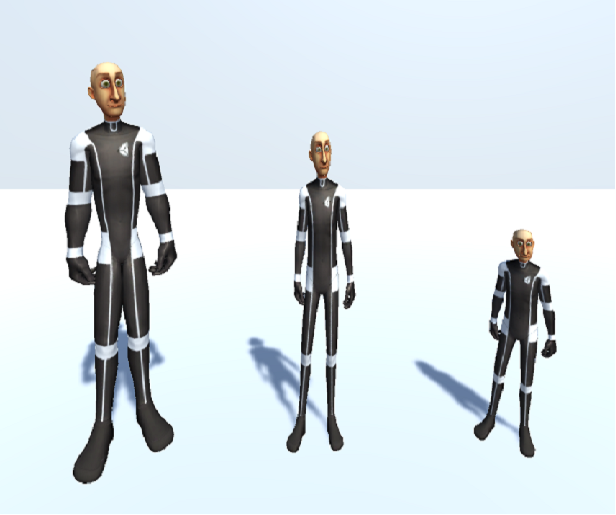
\includegraphics[width=0.31\textwidth]{images/LevelOfHomogeneity.png} \\
	(a) & (b) & (c)
	\end{tabular}
	\caption{\label{fig:crowd-parameter-ex}Crowd configuration and simulation: a) High Level of service, b)Low level of service, c)Level of Homogeneity}
\end{figure*}

\begin{table}
	\centering
	\begin{tabular}{||c c ||}
		\hline
		LOS & Crowd Density (people/square unit)\\ [0.5ex] 
		\hline\hline
		A & $<$=0.27  \\ 
		\hline
		B & 0.31 - 0.43 \\
		\hline
		C & 0.44 - 0.72  \\
		\hline
		D & 0.72 - 1.08 \\
		\hline
		E & 1.09 - 2.17 \\
		\hline
		F & $>$ 2.17 \\ 
		\hline
	\end{tabular}
	\caption{LoS classifications and their associated densities.}
	\label{table:los}
\end{table}

We formally denote a crowd $C = \langle g, k, l \rangle$ that describes the crowd related parameters where g, k, l denote LoS, LoA, LoH respectively.
A gamified environment area is formally described as multiple heterogeneous sub areas. Let $y_{j}$ be a random variable for sub area j with a value in range [$g_{min},g_{max}$]. Let, $n_{j}$ be the number of members in the sub area j.

\begin{equation}
\mathbf{n_{j}} = Q_{j} \times \delta \times x_{i} 
\end{equation}

where, $Q_{j}$ is the area of sub area j and $\delta$ is the normalization constant.
We described a transformation/mapping function that converts the crowd configuration to an instance of member $A = \{ a \}$ where each member $a = \langle \mathbf{p}, \mathbf{v},\mathbf{f}, \mathbf{r},\mathbf{h},\mathbf{m} \rangle$ where p = position vector ($\hat{x_{a}},\hat{y_{a}},\hat{z_{a}}$), v = speed, r = radius, h = height, f = acceleration. $\hat{x_{a}}$ and $\hat{z_{a}}$ are random variables in range [$x_{min_{j}}$,$x_{max_{j}}$] and [$z_{min_{j}}$,$z_{max_{j}}$] respectively where $x_{min_{j}}$,$x_{max_{j}}$,$z_{min_{j}}$,$z_{max_{j}}$ are the four extreme coordinates of sub square area j.

\begin{table}
\centering
	\begin{tabular}{||c c c ||} 
	\hline
	k & $x_{i}$ & $v_{a}$\\ [0.5ex] 
	\hline\hline
	Low & $<$=0.7 & $S+ SLOW\times x_{i}$ \\ 
	\hline
	Low & $>$0.7 & $S+ SHIGH\times x_{i}$\\
	\hline
	Medium & $<$=0.5 & $S+ SLOW\times x_{i}$ \\
	\hline
	Medium & $>$0.5 & $S+ SHIGH\times x_{i}$\\
	\hline
	High & $<$=0.7 & $S+ SHIGH\times x_{i} $\\
	\hline
	High & $>$ 0.7 & $S+ SLOW\times x_{i}$\\
	\hline
	\end{tabular}
	\caption{\label{table:aggression-levels-speeds} Speed mapping for aggression levels. Let, $x_{i}$ be the random variable for member i whose value is in the range [0,1]. SLOW and SHIGH are higher and lower aggression factors for speed respectively. S is the speed constant.}
\end{table}

\begin{table}
\centering
	\begin{tabular}{||c c c ||} 
	\hline
	k & $x_{i}$ & $f_{a}$\\ [0.5ex] 
	\hline\hline
	Low & $<$=0.7 & $F+ ALOW\times x_{i}$ \\ 
	\hline
	Low & $>$0.7 & $ F+ AHIGH\times x_{i} $\\
	\hline
	Medium & $<$=0.5 & $F+ ALOW\times x_{i}$ \\
	\hline
	Medium & $>$0.5 & $F+ AHIGH\times x_{i}$\\
	\hline
	High & $<$=0.7 & $F+ AHIGH\times x_{i} $\\
	\hline
	High & $>$ 0.7 & $F+ ALOW\times x_{i}$\\
	\hline
	\end{tabular}
	\caption{\label{table:aggression-levels-accels} Acceleration mapping for aggression levels. ALOW and AHIGH are higher and lower aggression factor for acceleration respectively. F is the acceleration constant.}
\end{table}

Formally, Level of Homogeneity is defined in terms of M,H,R as each crowd member's mass, height, and radius respectively. 
Let $ \alpha , \beta, \gamma $ be heterogeneity factor for mass, height and radius respectively.  The mapping of level to these factors can be found in Table~\ref{table:homogeneity-levels}.

\begin{table}
\centering
	\begin{tabular}{||c c c c c||} 
	\hline
	l & $x_{i}$ & $m_{a}$ & $h_{a}$ & $r_{a}$\\ [0.5ex] 
	\hline\hline
	Low & $<$=0.7 & $M\times \alpha \times x_{i} $ & $h\times \beta \times x_{i}$ & $r\times \gamma \times x_{i} $ \\ 
	\hline
	Medium & $<$=0.5 & $ M\times \alpha \times x_{i}$ & $h\times \beta \times x_{i}$ & $r\times \gamma \times x_{i}$\\
	\hline
	High & $<$=0.3 & $M\times \alpha \times x_{i}$ & $h\times \beta \times x_{i} $ & $r\times \gamma \times x_{i} $\\
	\hline
	\end{tabular}
	\caption{\label{table:homogeneity-levels} Height, radius, and mass mapping for aggression levels.}
\end{table}

%%%%%%%%%%%%%%%%%%%%%%%%%%%%%%%
\section{Crowd-Aware Environment Analysis}
\label{section-crowdenv}
\begin{figure*}
	\begin{tabular}{c c c c c}
	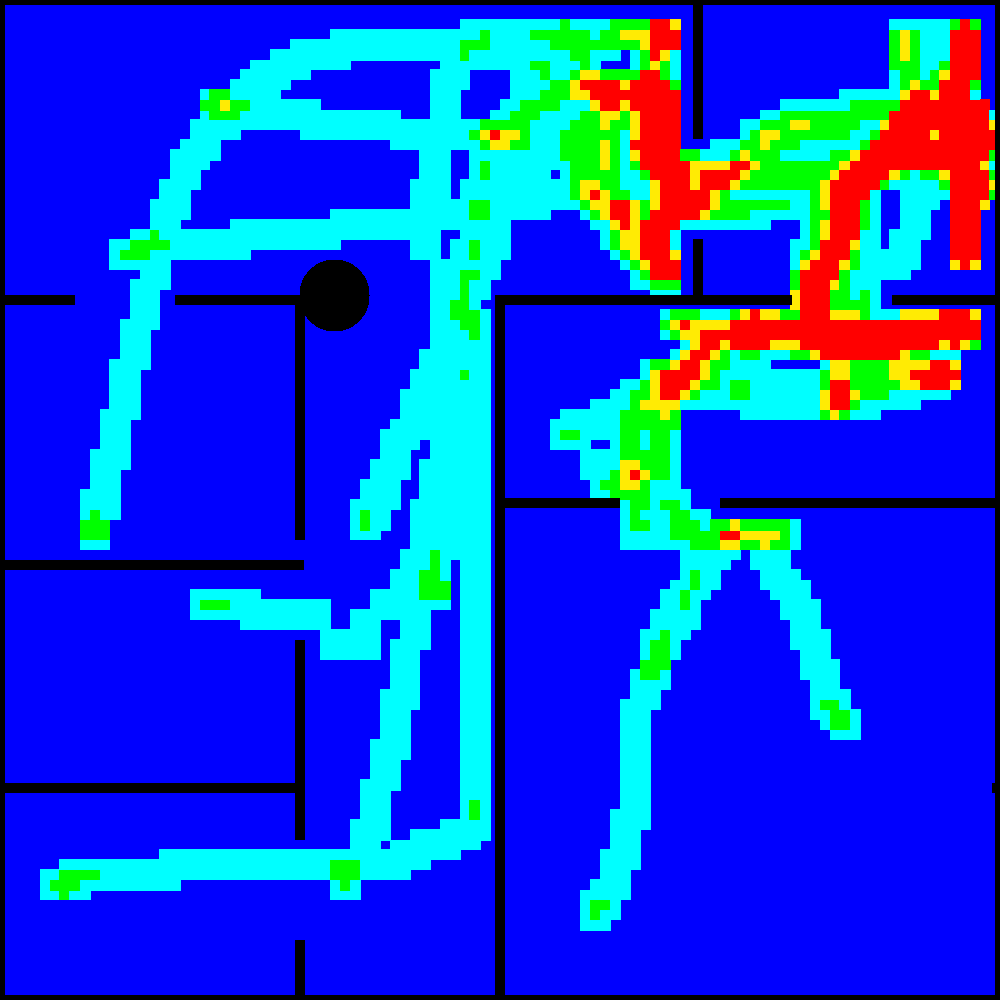
\includegraphics[width=0.19\textwidth]{images/Hypothesis1/Iter1-User-17_t_16_615.png} & 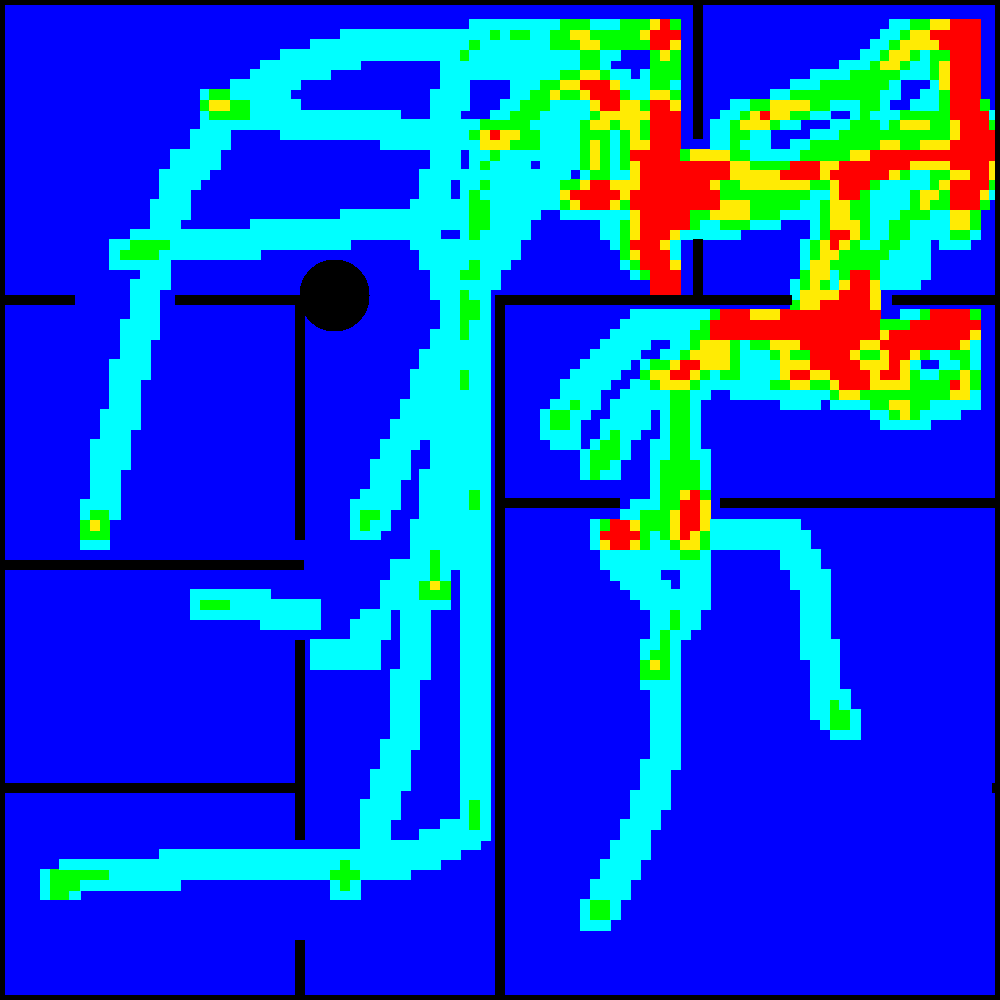
\includegraphics[width=0.19\textwidth]{images/Hypothesis1/Iter2-User-17_t_12_738.png} & 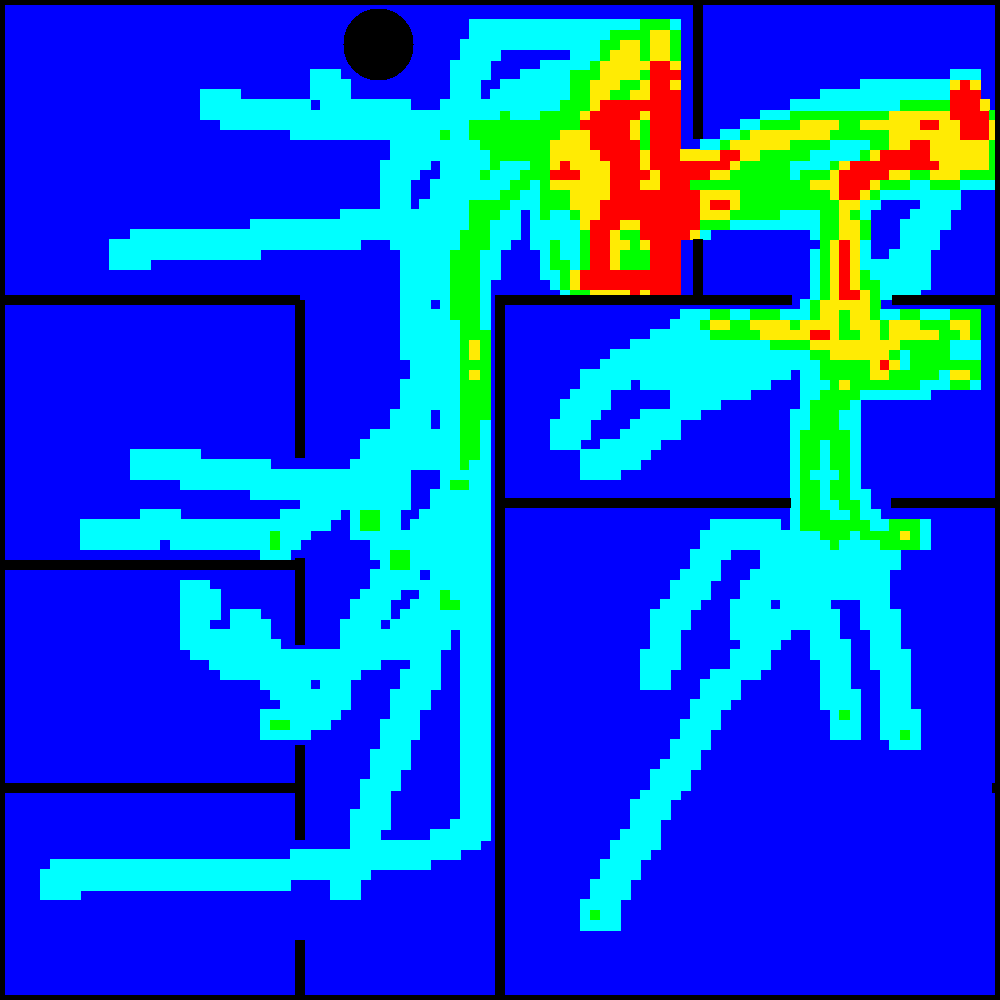
\includegraphics[width=0.19\textwidth]{images/Hypothesis1/Iter3-User-17_t_10_692.png} & 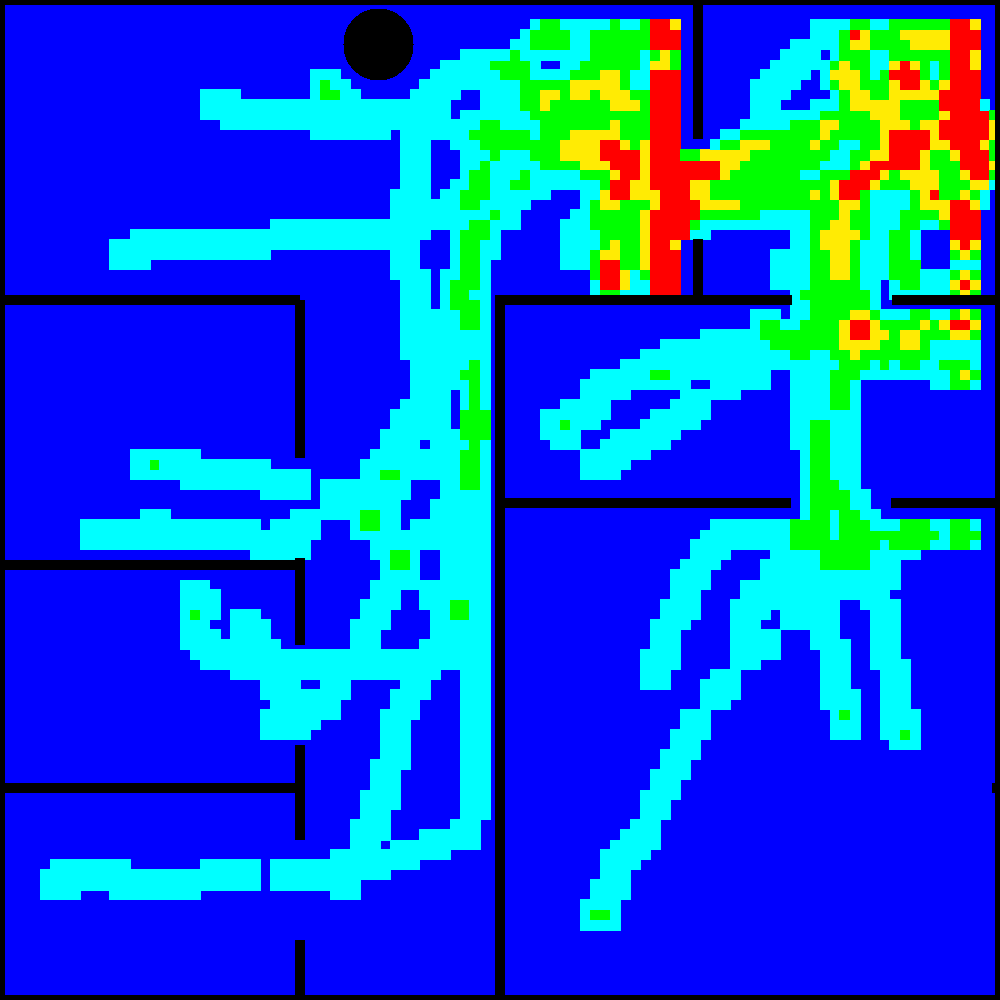
\includegraphics[width=0.19\textwidth]{images/Hypothesis1/Iter4-User-17_t_9_323.png} & 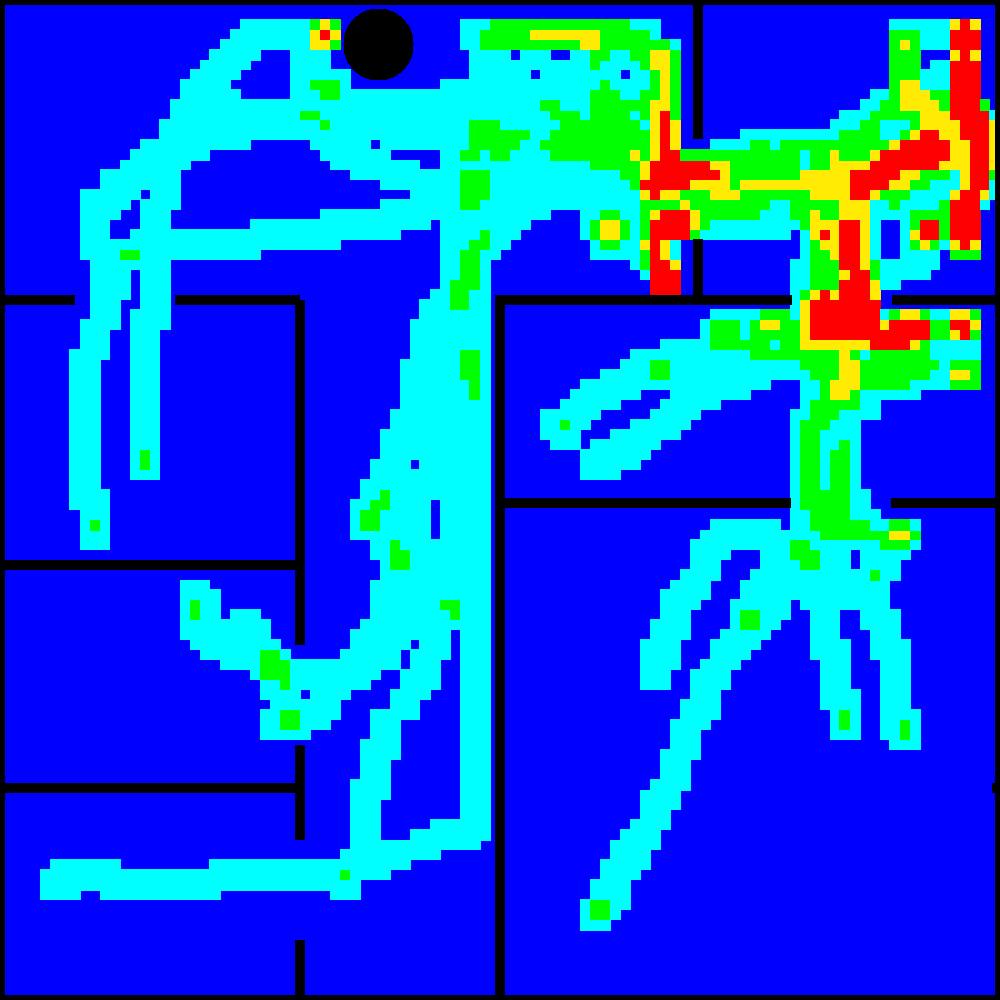
\includegraphics[width=0.19\textwidth]{images/Hypothesis1/Iter5-User-17_t_9_174.png} \\
	(a) & (b) & (c) & (d) & (e)\\
	Time=16.615 & Time= 12.738 & Time=10.692 & Time=9.323 & Time=9.174
	\end{tabular}
	\caption{\label{fig:single-player-iterative-improvement}Iterative environment improvement, in terms of evacuation time, is shown from left to right.}
\end{figure*}

A suite of analysis tools are made available to a player in order to visually validate their simulation results.  In particular we visualize metrics using heatmap so that the user can improve their design by identifying regions which are not performing well. The heat map is an orthographic view of the design containing all the elements(walls, doors,pillars) placed by the user and the path of all the agents. The level of crowd density of a region in the layout can be deduced by different coloured dots in the heat map. Figure~\ref{fig:single-player-iterative-improvement} is an example of a heat map which shows the orthographic view of walls, doors, and pillars in the layout with aggregate crowds dynamics displayed as heat traces. If a region is not performing well, it will become congested and crowd density will rise and the region will become more red. A player can be improve the design to reduce the highlighted areas in the design.




%%%%%%%%%%%%%%%%%%%%%%%%%%%%%%%
\section{Competitive Co-design of Environments}
\label{section-IterEnv}
The game framework supports optimal environment design through an iterative and entertaining approach. A player can improve their design to reach optimality by iterating on subtle design modifications and running simulations.  Furthermore, the framework supports collaboration and competitive co-design by exposing players to other's designs and performance analyses.

We have also provided the user the ability to reinforce their design by learning from the best player's moves. One way that this is achieved is to show the best scorer's heatmap. A player can gain knowledge from that heatmap to potentially incrementally improve their design. By allowing players to iteratively replay and view other's analyses and designs the game fosters collaboration in our game which can guide player's to a more optimal architectural design.

%%%%%%%%%%%%%%%%%%%%%%%%%%%%%%%
\section{Evaluation}
\label{section-results}
We hypothesize that with the gamification of a complex combinatorial problem in architectural design provides a user an innovative means to improve their design and gradually reach optimality. We also hypothesize that competitive co-design is an effective solution to the non-convex optimization problem that is crowd-aware environment design for efficient evacuation. We have conducted some user studies below to evaluate our hypothesis.

\subsection{User Study}
For our first hypothesis, we evaluated the evacuation times of certain user iterations for each of the 54 combinations of crowd configuration parameters. We have considered only the data of an user who has viewed the heat map for every iteration. For the second hypothesis, for each of the game level and each of the crowd parameter combination we have plotted all the evacuation times of user simulation runs in order of time of execution. We have considered the data of the users who have viewed the best scorer's heat map. 

Each player is identified by a unique id assigned to him/her. Some of the user data we gathered are Player id, User placed architectural element positions, Total evacuation time of the simulation, User choices of crowd configuration parameters (LoS, LoA, LoH), User's choice of viewing the heat map, User's choice of viewing the Top Scorer's heat map. 

\subsubsection{Procedure}
We have provided the user an existing layout at the start of the level which helps us increase the difficulty as the user gradually reaches higher levels. Users cannot manipulate these already placed elements. Users can create a wall by clicking on two points in the layout. Pillars can be created by clicking at a point, on the floor, where the player want to place the pillar. The radius of the pillar can be changed by playing around with the slider in the creation menu. Doors can be created by clicking on the walls where the user wants to place the door. Walls, doors and pillars created by the user can be deleted by selecting them again. There are keyboard keys assigned to increase or decrease the width of the wall to be placed. Walls can be moved around by clicking them and using the arrows keys or by dragging them with the use of a mouse.

There are several constraints associated with each element in the layout. First of all the users cannot modify the elements of the layout existing when the level started. Users can only manipulate the elements they added to the existing layout. There are a fixed number of walls, pillars and doors that can be placed by the user.  Walls can be placed only if it forms an enclosed space meaning that a wall must be touching walls on either end. A wall cannot be made to pass through the outside wall. In case the wall is placed incorrectly by the player, the wall will be marked red, and the player will not be able to start the simulation until the errors are rectified. If the width of the wall is less than two units, the wall will not be created.

\begin{figure*}[ht] 
\centering
\begin{tabular}{c c c c c}
	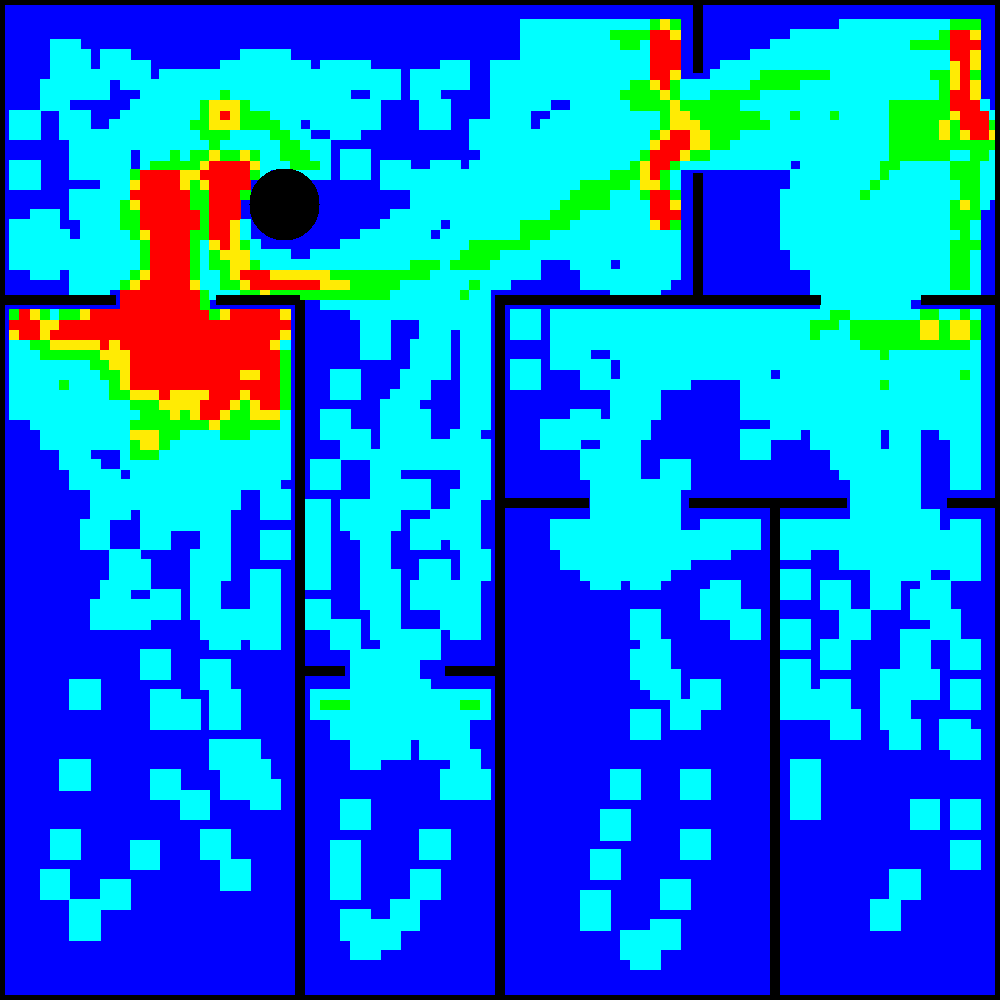
\includegraphics[width=0.19\textwidth]{images/Hypothesis2/Iter1-ID-12_t_16_4175.png} & 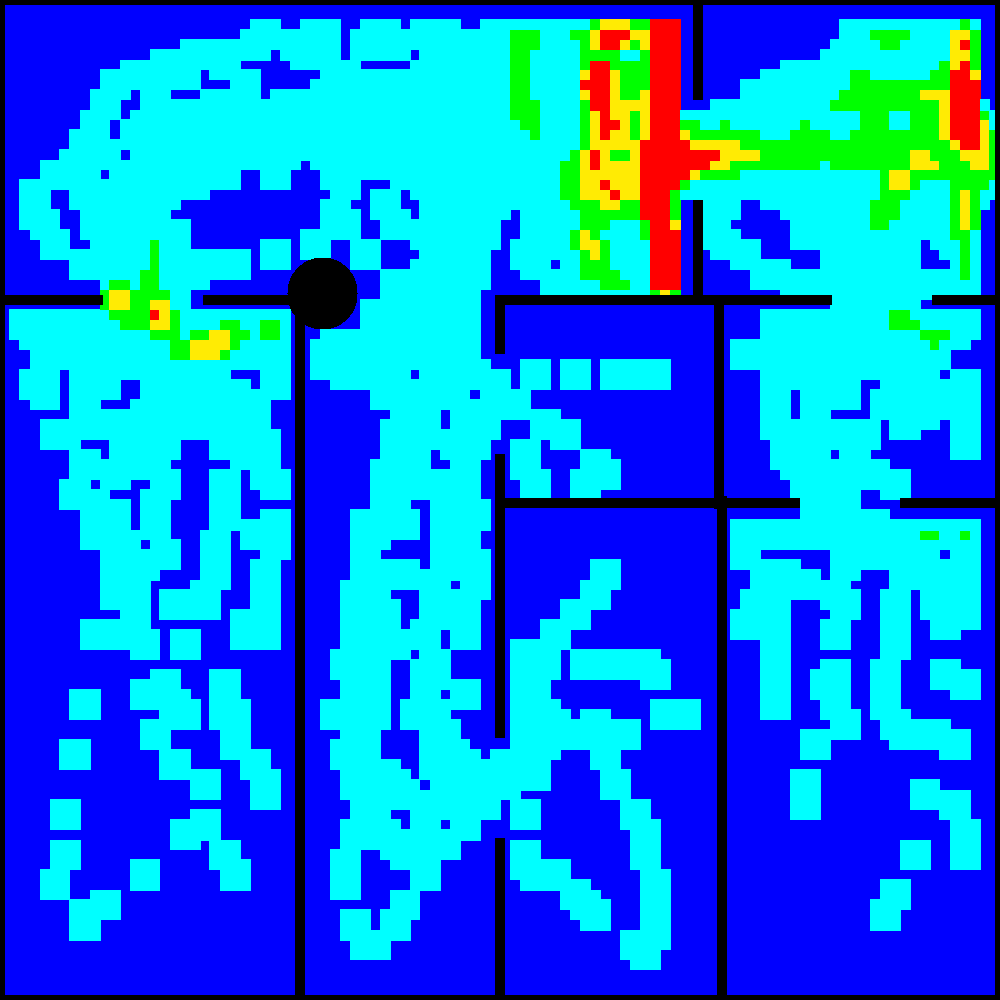
\includegraphics[width=0.19\textwidth]{images/Hypothesis2/Iter2-ID-8_t_13_695.png} & 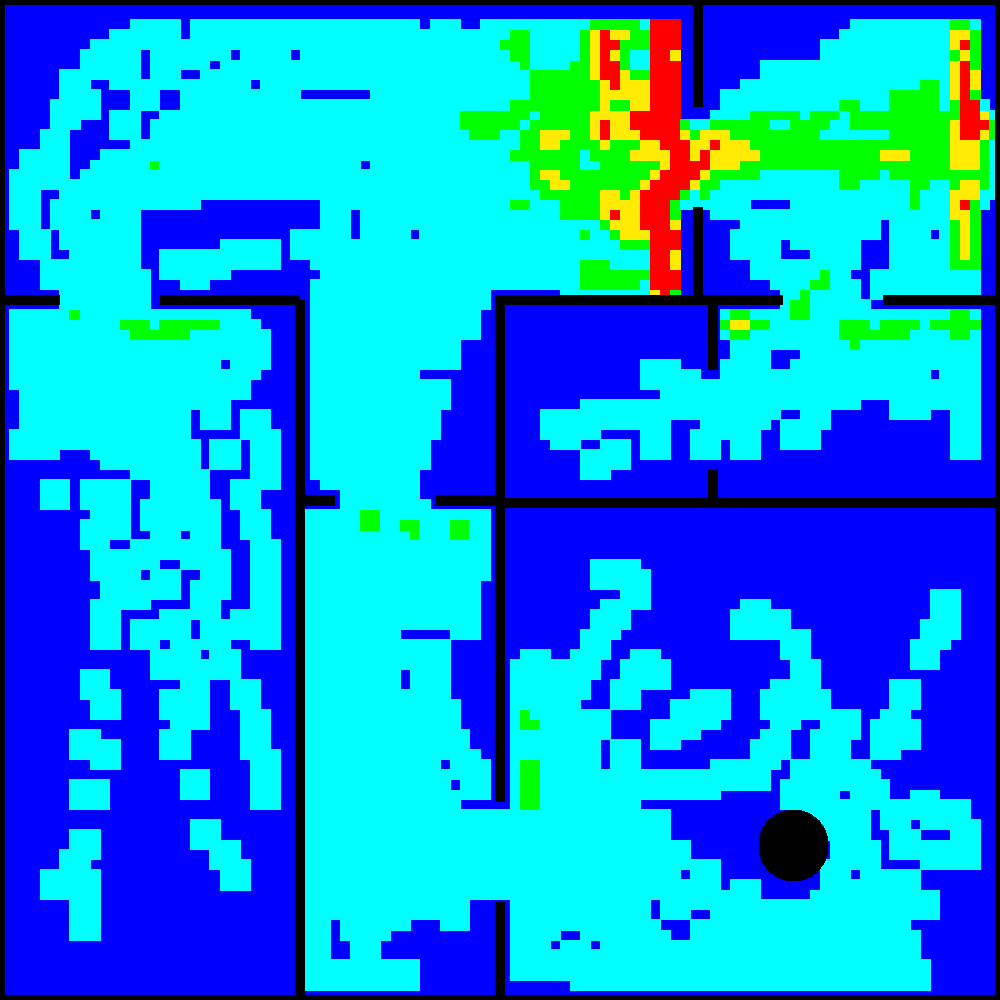
\includegraphics[width=0.19\textwidth]{images/Hypothesis2/Iter3-ID-22-t_11_1705.png} & 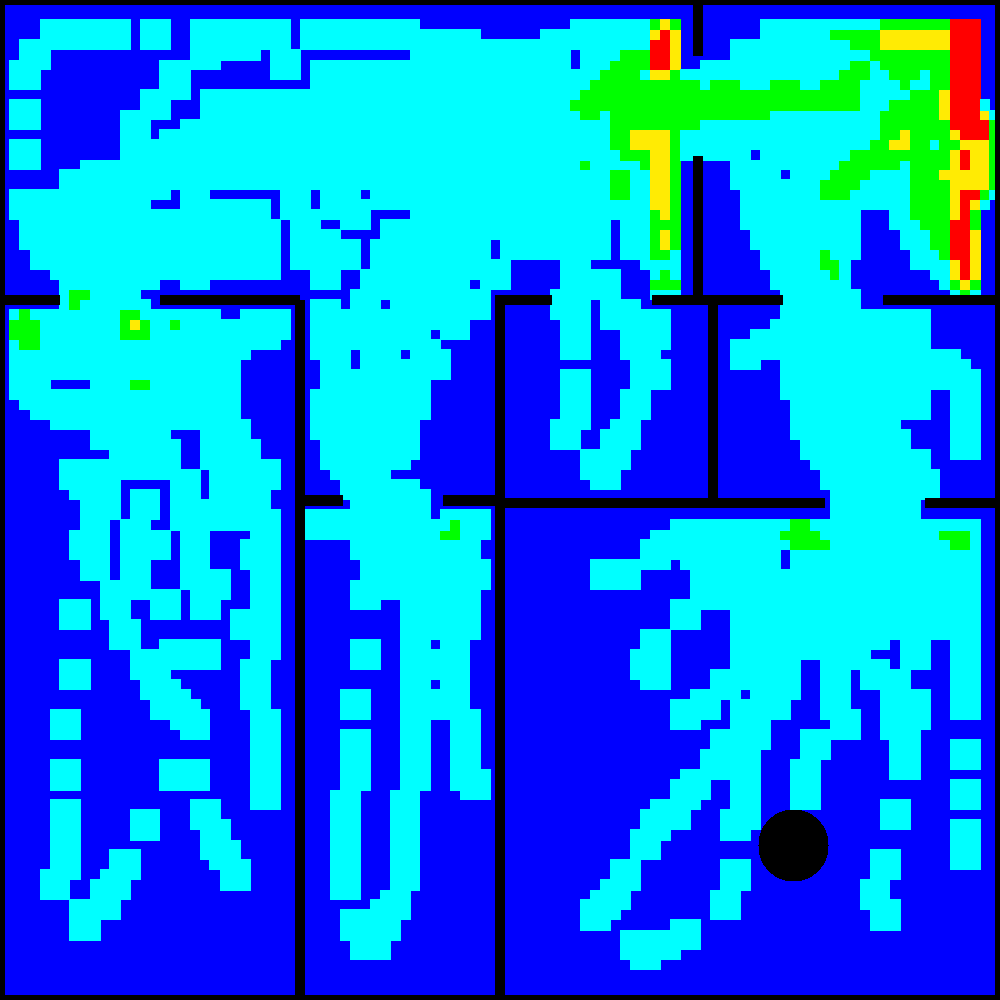
\includegraphics[width=0.19\textwidth]{images/Hypothesis2/Iter4-ID-17-t_9_669.png} & 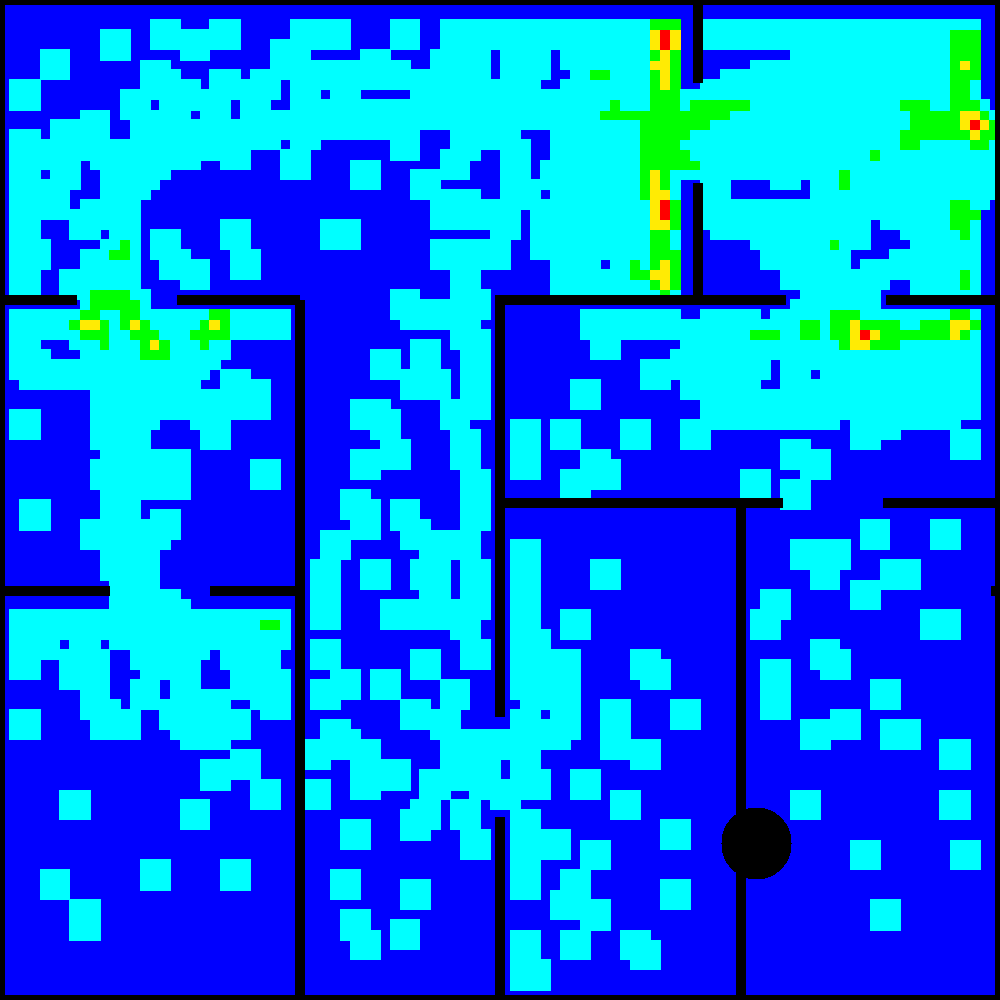
\includegraphics[width=0.19\textwidth]{images/Hypothesis2/Iter6-ID-17-t_8_151.png} \\
	Time=16.4175 & Time=13.695 & Time=11.1705 & Time=9.669 & Time=8.151
\end{tabular}
  \caption{\label{fig:codesign-incremental-improvement}Current best player's heatmap with  evacuation time for the crowd configuration LoS=F,LoA=High,LoH=Low in level 1}
  \begin{tabular}{c c c }
	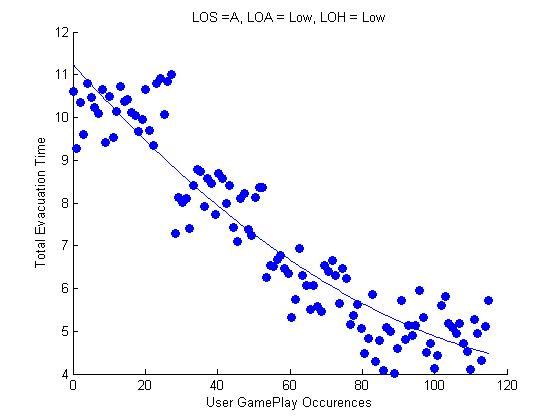
\includegraphics[width=0.31\textwidth]{images/Hypothesis2Graphs/LOS_A_LOA_Low_LOH_Low.jpg} &  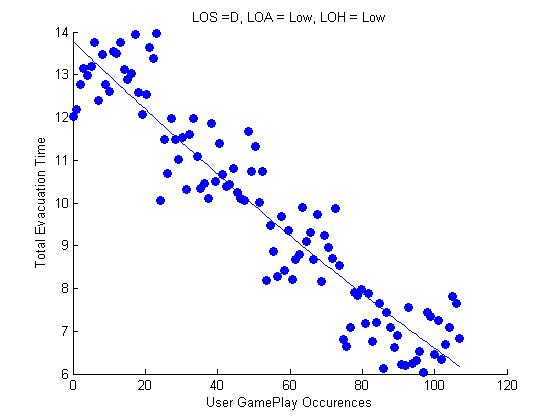
\includegraphics[width=0.31\textwidth]{images/Hypothesis2Graphs/LOS_D_LOA_Low_LOH_Low.jpg} &  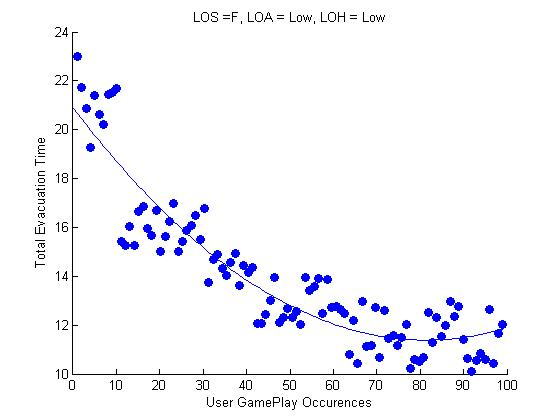
\includegraphics[width=0.31\textwidth]{images/Hypothesis2Graphs/LOS_F_LOA_Low_LOH_Low.jpg} \\
	LOS=A,LOA=Low,LOH=Low & LOS=D,LOA=Low,LOH=Low & LOS=F,LOA=Low,LOH=Low
\end{tabular}
  \caption{\label{fig:codesign-heatmap-changes}the Graphs of Evacuation Times for different User Gameplays in order of occurrence for 3 different combinations of crowd configuration parameters}
\end{figure*}

\subsection{Results}
In order to evaluate our hypotheses, we hosted our game on our website and asked people to play the game. We collected data for different users and for different levels. Analysing and comparing the results, we observed the following.

After analyzing the evacuation times of each user iterations for each level and each combination of crowd configurations, we have found a gradually decreasing curve of evacuation time in 73.33\% of total 60 user cases. In Figure~\ref{fig:single-player-iterative-improvement} we demonstrate a single case of iterative improvement of a design by a player using the crowd configuration Los=crowd density of 1.09-2.17, LoA=High, LoH=Low.To prove that we used the following method.

For each user we have calculated the following and plotted.
    \begin{equation}
\sum_{i=1}^{n_{A}-1} I(i+1,i)
 \end{equation}
    
    where, $n_{A}$ is the total number of iterations by an user A and
    
    \begin{equation*}
I(i+1,i) = \begin{cases}
1 &\text{$E_{i+1}$ - $E_{i}$ < 0.1}\  \\  -1 &\text{$E_{i+1}$-$E_{i}$ $\geq$ 0.1}
\end{cases}
\end{equation*}
where, $E_{i}$ is the evacuation time of user A's $i^{th}$ iteration. The threshold of difference in evacuation time between two consecutive iterations for a positive case is 0.1. We have then plotted the summation values from equation (2) for each user shown in histogram ~\ref{fig:histogram-of- positive-use-cases}. The bars beyond the 0, represents number of positive cases and the rest are number negative cases.

\begin{figure}
\centering
	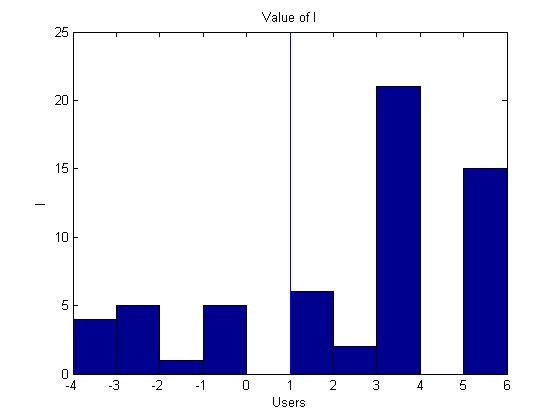
\includegraphics[width=0.3\textwidth]{images/ValueofI-Histogram.jpg} 
  \caption{\label{fig:histogram-of- positive-use-cases}The bars represents number of user. The positive user cases are beyond 0}
\end{figure}


For the second hypothesis, it was found that the evacuation times of different players viewing the current best scorer's heat map, gradually decreased and converged towards optimality. The curve formed by these players is very similar to that of a fitness function in computational optimization strategies. Figure~\ref{fig:codesign-incremental-improvement} is an example of this curve in which several player's iteratively improved a design by using the current best player's analyses and environment layout information. The Figure~\ref{fig:codesign-heatmap-changes} shows the Graphs of Evacuation Times for different User Gameplays in order of occurrence for 3 different combinations of crowd configuration parameters. 



\subsection{System Usability Results}
We are using the System Usability Scale to calculate the System Usability Scale(SUS) score~\cite{JBrookeSUS}. We received feedback from 61 players and calculated the score depending upon their responses. Our average usability score is 78.69 out of a scale of 100. Hence, our usability is average but there is a lot of scope for improvement.










%%%%%%%%%%%%%%%%%%%%%%%%%%%%%%%
\section{Conclusion}
\label{section-conclusion}
Some of the short comings of our current game was that some of the levels were quite tedious. Layouts in each level are designed manually. It would much more effective if this process was automated. All agents behavior in the game is quite similar and it would make sense to provide different behaviors to different agents. The game also needs more advanced architectural standards to be included as constraints to help casual users' designs to meet these standards. Future work includes making the simulations as realistic as possible with improved agent behavior. Users can be provided with behavior elements to add to their crowd agents along with the current crowd configuration parameters.

We think that our game can help the knowledge of architectural design go beyond the boundaries of architectural experts and can make the task of architectural design more interesting and entertaining. We also believe this paper is a beginning of more future architectural researches using serious games.
 

 

\balance{}

% References must be the same font size as other body text.
\bibliographystyle{SIGCHI-Reference-Format}
\bibliography{paper}

\end{document}